\documentclass[12pt,a4paper]{article}
\usepackage{pdfpages}
% (fold)
\usepackage{booktabs,amsmath,multirow} 
\usepackage{mathtools} % needed for next line
\mathtoolsset{showonlyrefs}
\usepackage{fullpage}
 % only shows number of referenced equations
% \newcommand{\dpder}[3][]{\dfrac{\partial^{#1}#2}{\partial #3}} \addtolength{\oddsidemargin}{-.875in} \addtolength{\evensidemargin}{-.875in} \addtolength{\textwidth}{1.75in}
% \addtolength{\topmargin}{-.875in} \addtolength{\textheight}{1.75in}

% need for subequations
\usepackage{graphicx} 

% need for figures
\usepackage{verbatim}

% useful for program l,istings
\usepackage{color} 

% use if color is used in text
\usepackage{subfigure}
\newcommand{\+}[1]{\ensuremath{\mathbf{#1}}}
% use for side-by-side figures
\usepackage[pdfpagemode={UseOutlines},bookmarks=true,bookmarksopen=true, bookmarksopenlevel=0,bookmarksnumbered=true,hypertexnames=false, colorlinks,linkcolor={blue},citecolor={blue},urlcolor={red}, pdfstartview={FitV},unicode,breaklinks=true]{hyperref} 
\graphicspath{ {Figures/}{Tables/}}
% use for hypertext links, including those to external documents and URLs
\newcommand{\ajp}{AJP} 
\newcommand{\ig}{ 
\includegraphics} 
\newcommand{\tu}{\textup} \hypersetup{urlcolor=blue, colorlinks=true} 
\usepackage[square, numbers, comma, sort&compress,super]{natbib}
% Colors hyperlinks in blue - change to black if annoying
% don't need the following. simply use defaults
\setlength{\baselineskip}{16.0pt} 

% 16 pt usual spacing between lines
\begin{comment}
	\pagestyle{empty} 
	
	% use if page numbers not wanted
\end{comment}

% Specifies the directory where pictures are stored
% above is the preamble (end)
\def\MyWidth{.71\textwidth} % textwidth for multiple graphs
\begin{document} 
\title{Kalman Filtering} 
\author{Kevin Mead}

%\affiliation{KTH Royal Institute of Technology, Electrotechnical Modelling} \email{kmead@kth.se}
\date{\today} 
\maketitle 
%!TEX root = /Users/kevin/SkyDrive/KTH Work/Period 4 2014/GNSS/Labs/L4 - Kalman filtering/main.tex

\section{Introduction} 

% (fold)
\label{sec:introduction}  The task is to compute the coordinates and velocities of a moving vehicle.  The calculations were done with a constant velocity kinematic model.  Measurement values in the Excel document, \emph{Measurement.xls}, give us the position and speed of the vehicle measured in 2 second intervals.  Other values given are:
\begin{itemize}
	\item[-]PSD (power spectral density) of the random acceleration: $0.01~\mathrm{m}^2\mathrm{s}^{−3}$
	\item[-]Standard deviation of measured coordinates (both components): $3~\mathrm{m}$
	\item[-]Standard deviation of measured abs. velocity: $0.5~\mathrm{m}/\mathrm{s}$
	\item[-]Standard deviation of initial velocity (both components): $3~\mathrm{m}/\mathrm{s}$
	\item[-]Standard deviation of initial coordinates (both components): $10~\mathrm{m}$
\end{itemize}

% section introduction (end)

% Write a standard report, which should include:
% - Description of the surveying procedure
% - Description of the processing procedure
% - Screen dump from Google Earth showing your detail measurements
% - Screen dump from Trimble Business Center showing the terrain model in 3D view
% - Processing baselines KTH – DUB2 (or 17), KIRU – DUB2 (or 17): comparison and
% discussion
%!TEX root = /Users/kevin/SkyDrive/KTH Work/Period 4 2014/GNSS/Labs/L4 - Kalman filtering/main.tex

\section{Methodology} 

% (fold)
\label{sec:methodology}

% Describe the methods and instruments used to solve the problem. 
Matlab was used to solve for the following parameters and all of the following equations were taken from the technical report: Kalman Filtering.\cite{milanGPS} 
The steps and equations from the Kalman filtering algorithm are documented in the Matlab code. 
We start off with the matrix differential equation,
\begin{equation}
	\dot{\+x} (t) = \+F (t) x (t) + \+G (t) \+u (t) 
	\label{eq:eq1}
\end{equation} % (eq:eq1)
where $\+x = [${\rmfamily e~n~v$_e$~v$_n$}$]^{\mathrm{T}}$, the east and north positions and their velocity components. \+F, \+G, and \+u are given by,
\begin{equation}
	\begin{array}{ccc}
		\+F= \left[
		\begin{matrix}
			0 & 0 & 1 & 0 \\
			0 & 0 & 0 & 1 \\
			0 & 0 & 0 & 0 \\
			0 & 0 & 0 & 0 \\
		\end{matrix}
		\right] & 
		\+G = \left[
		\begin{matrix}
			0 & 0 \\
			0 & 0 \\
			1 & 0 \\
			0 & 1 \\
		\end{matrix}
		\right] & 
		\+u = \left[
		\begin{matrix}
			\omega_{ae} \\
			\omega_{an} \\
		\end{matrix}
		\right] 
	\end{array}
\end{equation}
We do not know \+u because it represents white noise.  The discrete solution to Equation~\eqref{eq:eq1} is
\begin{equation}
	\+x_k = \+T_{k-1,k}\+x_{k-1} + \+w_{k-1,k}
	\label{eq:discreteSolutionToeq1}
\end{equation} % (eq:discretesolutiontoeq1)
where values of $k$ represent discretization of time. The transition matrix, $\+T_{k-1,k}$, can be approximated by,
\begin{equation}
	\+T_{k-1,k} = \+I + \+F_{k} \Delta t = \left[
			\begin{matrix}
				1 & 0 & \Delta t & 0 \\
				0 & 1 & 0           & \Delta t \\
				0 & 0 & 1           & 0 \\
				0 & 0 & 0           & 1 \\
			\end{matrix}
			\right]
	\label{eq:transitionMatrix}
\end{equation} % (eq:transitionmatrix)
The covariance of $\+w_k$, $\+Q_k$, is evaluated by use of the power spectral density (PSD) of the random acceleration, which are initially given. We can now represent the covariance of $\+w_k$ as,
\begin{equation}
	\+Q_k = \+Q_{G} \Delta t + (\+F \+Q_{G} + \+Q_{G} \+F^{\mathrm{T}})\frac{\Delta t^2}{2}
	+ \+F \+Q_{G} \+F^{\mathrm{T}} \frac{\Delta t^{3}}{3}
	\label{eq:eq12}
\end{equation} % (eq:covarianceqk)
where
\begin{equation}
	\begin{array}{cc}
		\+Q_{G} = \+G\+Q\+G^{\mathrm{T}} & \+Q = \left[
		\begin{matrix}
		q_{ae} 	& 0 		\\
		0		& q_{an} 	\\
		\end{matrix}
		\right]
	\end{array}
	\label{eq:eq11}
\end{equation} % (eq:q_g)


\subsection{Kalman Filter} % (fold)
\label{sub:kalman_filter}
The main steps of the discrete Kalman Filter algorithm are:
\begin{enumerate}
	\item Initialization:
	\begin{equation}
		\+x_0,~~\+Q_{x0} = \mathrm{var}[x_0]
		\label{eq:eq15}
	\end{equation} % (eq:eq15)
	\item Time propagation
	\begin{equation}
		\+x_k^- = \+T_{k-1,k}\+x_{k-1},~~\+Q_{x,k}^-= \+T_{k-1,k}\+Q_{x,k-1}\+T_{k-1,k}^{\mathrm{T}} + \+Q_k
		\label{eq:eq16}
	\end{equation} % (eq:eq16)
	\item Gain calculation:
	\begin{equation}
		\+K_k = \+Q_{x,k}^-\+H_k^{\mathrm{T}}[\+R_k+\+H_k \+Q_{x,k}^-\+H_k^{\mathrm{T}}]^{-1}
		\label{eq:eq17}
	\end{equation} % (eq:eq17)
	\item Measurement update
	\begin{equation}
		\+x_k = \+x_k^-+\+K_k[\tilde{L}_k-\+h_k(x_k^-)]
		\label{eq:eq18}
	\end{equation} % (eq:eq18)
	\item Covariance update
	\begin{equation}
		\+Q_{x,k} = [\+I-\+K_k \+H_k]\+Q_{x,k}^-
		\label{eq:19}
	\end{equation} % (eq:19)
\end{enumerate}
% subsection kalman_filter (end)
\subsection{Smoothing} % (fold)
\label{sub:smoothing}
After the Kalman Filter algorithm, we then smooth the results using the smoothed estimations for previous epochs,
\begin{equation}
	\hat{\+x}_k = \+x_k + \+D_k [\hat{\+x}_{k+1} - \+x_{k+1}^-]
	\label{eq:eq28}
\end{equation} % (eq:eq28)
\begin{equation}
	\+D_k = \+Q_{x,k}\+T_{k-1,k}^{T}(Q_{x,k+1}^-)^{-1}
	\label{eq:eq29}
\end{equation} % (eq:eq29)
with a covariance matrix of,
\begin{equation}
	\hat{\+Q}_{x,k} = \+Q_{x,k}+\+D_{k}[\hat{\+Q}_{x,k+1}-\+Q_{x,k+1}^-]\+D_k^{\mathrm{T}}
	\label{eq:eq30}
\end{equation} % (eq:eq30)
% subsection smoothing (end)

%!TEX root = /Users/kevin/SkyDrive/KTH Work/Period 4 2014/GNSS/Labs/L4 - Kalman filtering/main.tex


\section{Results} % (fold)
\label{sec:results}
A comparison of the filtered and smoothed coordinates with the true measurements are shown in Figures~\ref{fig:Figures_xDataPlots} and \ref{fig:Figures_vDataPlots}. Table~\ref{tab:tableFiltered.tex} and~\ref{tab:tableSmoothed.tex} are the coordinates after filtering and smoothing.  Figures~\ref{fig:Figures_diffPlots} and \ref{fig:Figures_diffPlotsVelocity} show the difference between the true measurements and the filtered and smoothed results.
\begin{figure}[htbp]
	\centering
		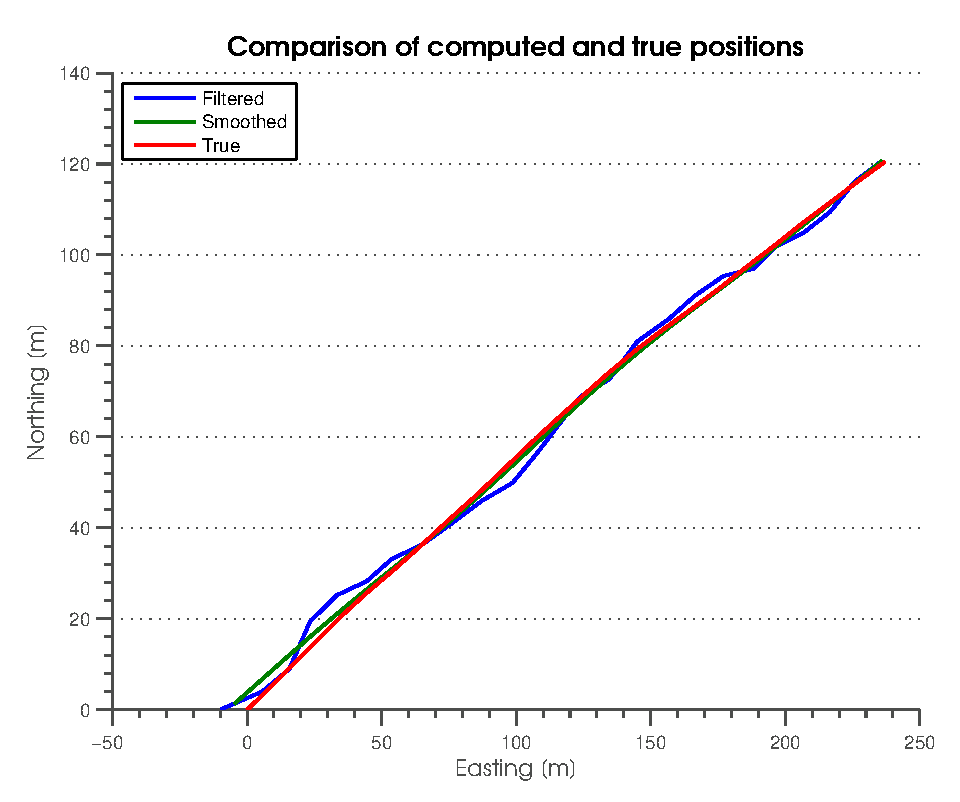
\includegraphics[width=\MyWidth]{Figures/xDataPlots.eps}
	\caption{Comparison of filtered, smoothed, original, and true coordinates.}
	\label{fig:Figures_xDataPlots}
\end{figure} % (fig:Figures_xDataPlots)
\begin{figure}[htbp]
	\centering
		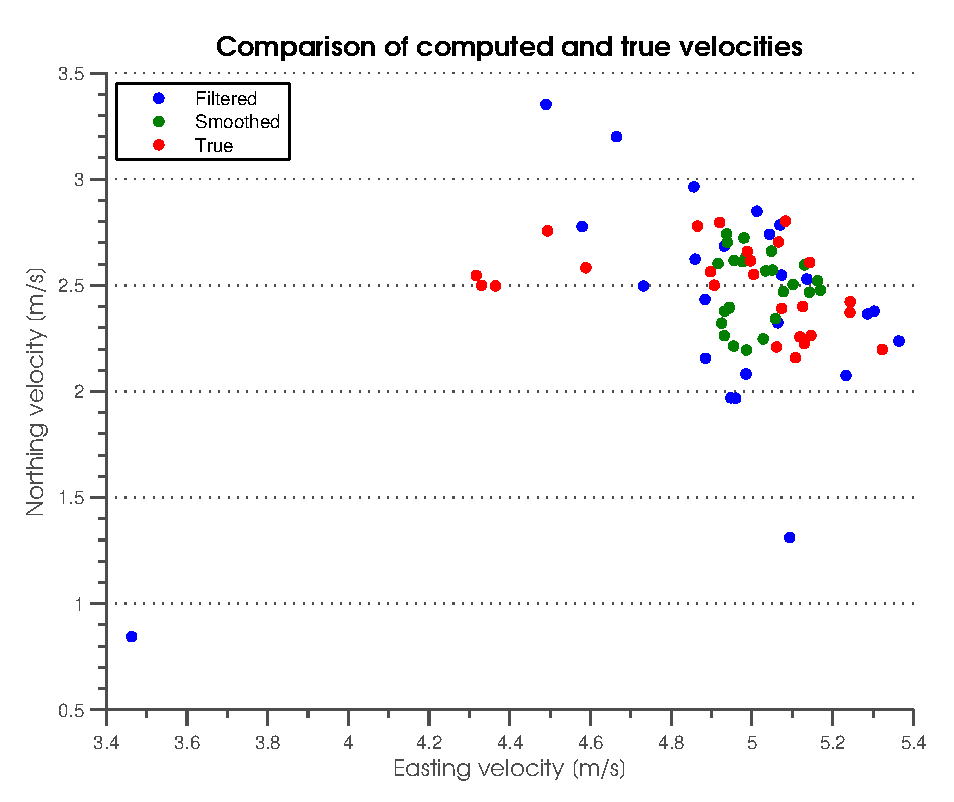
\includegraphics[width=\MyWidth]{Figures/vDataPlots.eps}
	\caption{Comparison of filtered, smoothed, and true velocities.}
	\label{fig:Figures_vDataPlots}
\end{figure} % (fig:Figures_vDataPlots)
\begin{table}[h] 
   \begin{center} 
      \begin{tabular}{lllllllll}\toprule 
\multicolumn{5}{c}{Filtered Estimations and standard deviations}\\ 
\midrule 
t&  $x_e \pm \sigma_e$& $x_n \pm \sigma_n$& $v_e \pm \sigma_{v_e}$& $v_n \pm \sigma_{v_n}$\\ \midrule 
0 & $   -9.62 \pm    10.00$ & $    0.11 \pm    10.00$ & $    3.46 \pm     3.00$ & $    0.84 \pm     3.00$  \\ 
2 & $    5.71 \pm     1.71$ & $    4.00 \pm     1.71$ & $    5.09 \pm     0.90$ & $    1.31 \pm     2.52$  \\ 
4 & $   15.74 \pm     1.33$ & $    8.98 \pm     1.64$ & $    4.95 \pm     0.51$ & $    1.97 \pm     1.05$  \\ 
6 & $   23.36 \pm     1.23$ & $   19.32 \pm     1.53$ & $    4.49 \pm     0.37$ & $    3.35 \pm     0.58$  \\ 
8 & $   33.40 \pm     1.19$ & $   25.17 \pm     1.42$ & $    4.66 \pm     0.30$ & $    3.20 \pm     0.40$  \\ 
10 & $   44.56 \pm     1.17$ & $   28.26 \pm     1.31$ & $    4.93 \pm     0.27$ & $    2.68 \pm     0.31$  \\ 
12 & $   53.82 \pm     1.15$ & $   33.15 \pm     1.24$ & $    4.86 \pm     0.25$ & $    2.62 \pm     0.27$  \\ 
14 & $   65.20 \pm     1.13$ & $   36.34 \pm     1.19$ & $    5.06 \pm     0.24$ & $    2.32 \pm     0.25$  \\ 
16 & $   76.79 \pm     1.11$ & $   41.27 \pm     1.16$ & $    5.30 \pm     0.23$ & $    2.38 \pm     0.24$  \\ 
18 & $   87.52 \pm     1.09$ & $   46.04 \pm     1.14$ & $    5.29 \pm     0.23$ & $    2.37 \pm     0.24$  \\ 
20 & $   98.70 \pm     1.09$ & $   49.89 \pm     1.13$ & $    5.36 \pm     0.23$ & $    2.24 \pm     0.24$  \\ 
22 & $  107.87 \pm     1.08$ & $   56.46 \pm     1.13$ & $    5.14 \pm     0.23$ & $    2.53 \pm     0.24$  \\ 
24 & $  117.40 \pm     1.08$ & $   63.85 \pm     1.13$ & $    5.01 \pm     0.23$ & $    2.85 \pm     0.24$  \\ 
26 & $  124.41 \pm     1.08$ & $   69.08 \pm     1.13$ & $    4.58 \pm     0.23$ & $    2.78 \pm     0.24$  \\ 
28 & $  134.62 \pm     1.08$ & $   72.63 \pm     1.13$ & $    4.73 \pm     0.23$ & $    2.50 \pm     0.24$  \\ 
30 & $  145.07 \pm     1.08$ & $   81.00 \pm     1.13$ & $    4.86 \pm     0.23$ & $    2.96 \pm     0.24$  \\ 
32 & $  156.58 \pm     1.08$ & $   85.84 \pm     1.13$ & $    5.07 \pm     0.23$ & $    2.78 \pm     0.24$  \\ 
34 & $  166.60 \pm     1.08$ & $   91.13 \pm     1.12$ & $    5.04 \pm     0.23$ & $    2.74 \pm     0.24$  \\ 
36 & $  177.15 \pm     1.08$ & $   95.37 \pm     1.12$ & $    5.07 \pm     0.23$ & $    2.55 \pm     0.24$  \\ 
38 & $  188.30 \pm     1.08$ & $   97.05 \pm     1.12$ & $    5.23 \pm     0.23$ & $    2.07 \pm     0.24$  \\ 
40 & $  196.25 \pm     1.08$ & $  101.75 \pm     1.13$ & $    4.89 \pm     0.23$ & $    2.16 \pm     0.24$  \\ 
42 & $  206.72 \pm     1.08$ & $  104.80 \pm     1.13$ & $    4.96 \pm     0.23$ & $    1.97 \pm     0.24$  \\ 
44 & $  216.74 \pm     1.08$ & $  109.52 \pm     1.13$ & $    4.99 \pm     0.23$ & $    2.08 \pm     0.24$  \\ 
46 & $  225.83 \pm     1.08$ & $  116.11 \pm     1.13$ & $    4.88 \pm     0.23$ & $    2.43 \pm     0.24$  \\ 
48 & $  236.10 \pm     1.08$ & $  120.72 \pm     1.13$ & $    4.94 \pm     0.23$ & $    2.39 \pm     0.24$  \\ \bottomrule 
      \end{tabular} 
   \end{center}
\caption{The easting and northing coordinates and velocities are given with their standard deviations.} 
\label{tab:tableFiltered.tex} 
\end{table} 

\begin{table}[h] 
   \begin{center} 
      \begin{tabular}{lllllllll}\toprule 
\multicolumn{5}{c}{Smoothed Estimations and standard deviations}\\ 
\midrule 
t&  $x_e \pm \sigma_e$& $x_n \pm \sigma_n$& $v_e \pm \sigma_{v_e}$& $v_n \pm \sigma_{v_n}$\\ \midrule 
0 & $    5.20 \pm     1.22$ & $    1.26 \pm     1.53$ & $    4.92 \pm     0.81$ & $    2.60 \pm     2.47$  \\ 
2 & $   15.13 \pm     0.42$ & $    6.48 \pm     0.37$ & $    4.96 \pm     0.37$ & $    2.62 \pm     0.97$  \\ 
4 & $   25.14 \pm     0.62$ & $   11.72 \pm     0.41$ & $    4.98 \pm     0.19$ & $    2.61 \pm     0.46$  \\ 
6 & $   35.28 \pm     0.62$ & $   16.90 \pm     0.37$ & $    5.03 \pm     0.07$ & $    2.57 \pm     0.24$  \\ 
8 & $   45.53 \pm     0.60$ & $   21.97 \pm     0.46$ & $    5.10 \pm     0.07$ & $    2.50 \pm     0.10$  \\ 
10 & $   55.84 \pm     0.59$ & $   26.94 \pm     0.53$ & $    5.14 \pm     0.10$ & $    2.47 \pm     0.08$  \\ 
12 & $   66.18 \pm     0.60$ & $   31.88 \pm     0.58$ & $    5.17 \pm     0.12$ & $    2.48 \pm     0.12$  \\ 
14 & $   76.48 \pm     0.61$ & $   36.87 \pm     0.61$ & $    5.16 \pm     0.12$ & $    2.52 \pm     0.13$  \\ 
16 & $   86.66 \pm     0.62$ & $   41.99 \pm     0.63$ & $    5.13 \pm     0.13$ & $    2.60 \pm     0.13$  \\ 
18 & $   96.69 \pm     0.63$ & $   47.24 \pm     0.65$ & $    5.05 \pm     0.13$ & $    2.66 \pm     0.13$  \\ 
20 & $  106.60 \pm     0.64$ & $   52.63 \pm     0.65$ & $    4.98 \pm     0.13$ & $    2.72 \pm     0.13$  \\ 
22 & $  116.47 \pm     0.64$ & $   58.11 \pm     0.65$ & $    4.94 \pm     0.13$ & $    2.74 \pm     0.13$  \\ 
24 & $  126.38 \pm     0.64$ & $   63.56 \pm     0.65$ & $    4.94 \pm     0.13$ & $    2.70 \pm     0.13$  \\ 
26 & $  136.43 \pm     0.65$ & $   68.90 \pm     0.65$ & $    4.98 \pm     0.13$ & $    2.64 \pm     0.13$  \\ 
28 & $  146.56 \pm     0.64$ & $   74.11 \pm     0.65$ & $    5.05 \pm     0.13$ & $    2.57 \pm     0.13$  \\ 
30 & $  156.71 \pm     0.65$ & $   79.17 \pm     0.65$ & $    5.08 \pm     0.13$ & $    2.47 \pm     0.13$  \\ 
32 & $  166.79 \pm     0.64$ & $   83.98 \pm     0.66$ & $    5.06 \pm     0.13$ & $    2.34 \pm     0.13$  \\ 
34 & $  176.81 \pm     0.65$ & $   88.56 \pm     0.66$ & $    5.03 \pm     0.13$ & $    2.25 \pm     0.13$  \\ 
36 & $  186.75 \pm     0.65$ & $   92.99 \pm     0.67$ & $    4.99 \pm     0.13$ & $    2.19 \pm     0.13$  \\ 
38 & $  196.63 \pm     0.65$ & $   97.39 \pm     0.67$ & $    4.95 \pm     0.13$ & $    2.21 \pm     0.14$  \\ 
40 & $  206.49 \pm     0.65$ & $  101.87 \pm     0.67$ & $    4.93 \pm     0.14$ & $    2.26 \pm     0.14$  \\ 
42 & $  216.34 \pm     0.67$ & $  106.45 \pm     0.68$ & $    4.93 \pm     0.15$ & $    2.32 \pm     0.15$  \\ 
44 & $  226.22 \pm     0.73$ & $  111.15 \pm     0.74$ & $    4.93 \pm     0.16$ & $    2.38 \pm     0.17$  \\ 
46 & $  236.10 \pm     0.85$ & $  115.93 \pm     0.88$ & $    4.94 \pm     0.19$ & $    2.40 \pm     0.20$  \\ \bottomrule 
      \end{tabular} 
   \end{center}
\caption{The easting and northing coordinates and velocities are given with their standard deviations.} 
\label{tab:tableSmoothed.tex} 
\end{table} 

\begin{figure}[h]
	\centering
		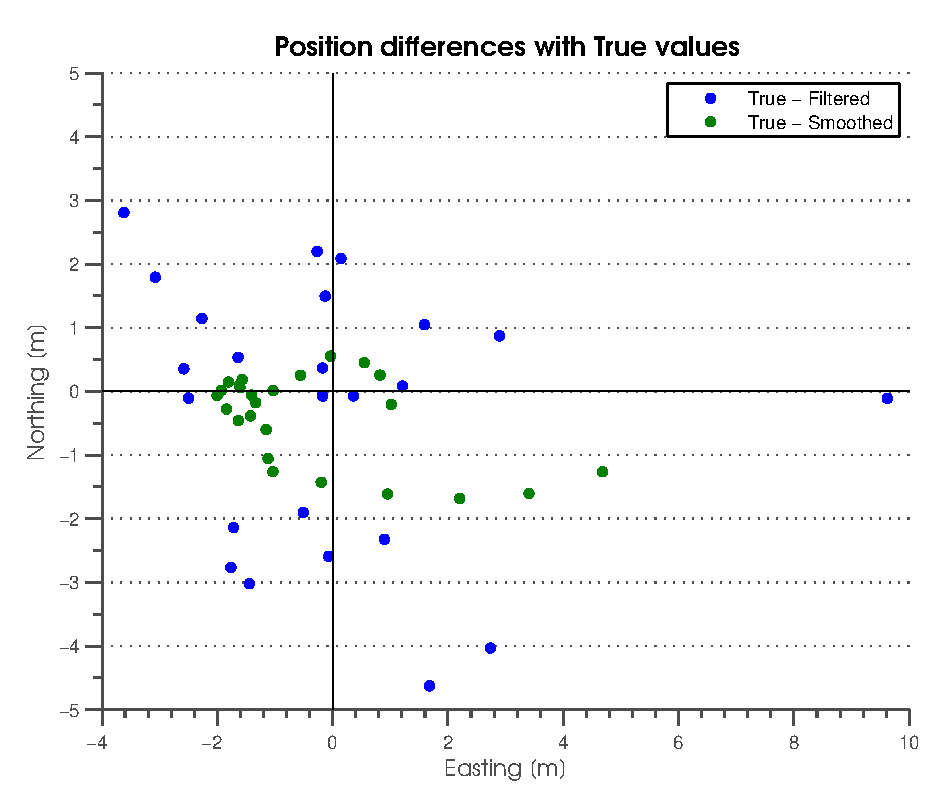
\includegraphics[width=\MyWidth]{Figures/diffPlots.eps}
	\caption{Plot of differences between true values and the filtered and smoothed coordinates.}
	\label{fig:Figures_diffPlots}
\end{figure} % (fig:Figures_diffPlots)
\begin{figure}[h]
	\centering
		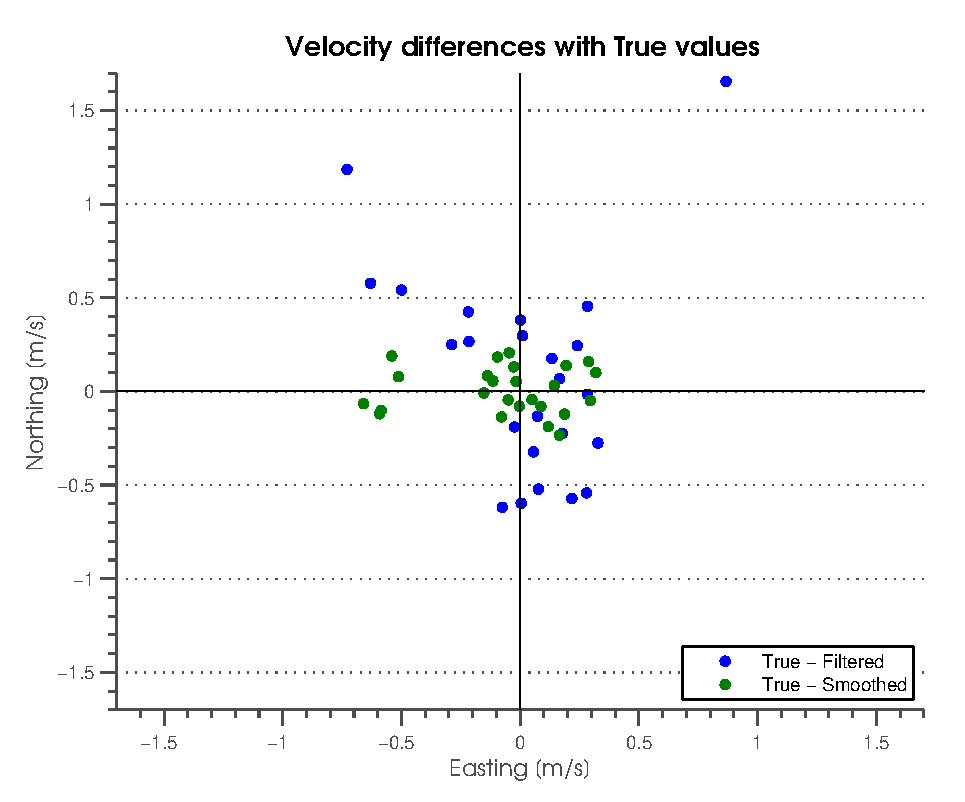
\includegraphics[width=\MyWidth]{Figures/diffPlotsVelocity.eps}
	\caption{Plot of differences between true values and the filtered and smoothed velocities.}
	\label{fig:Figures_diffPlotsVelocity}
\end{figure} % (fig:Figures_diffPlotsVelocity)
% section results (end)

%!TEX root = /Users/kevin/SkyDrive/KTH Work/Period 4 2014/GNSS/Labs/L4 - Kalman filtering/main.tex


\section{Analysis and Discussion} % (fold)
\label{sec:analysis_and_discussion}
% In this part you should discuss your results by, for example, considering the following questions:
\begin{itemize}
	\item Are the results reasonable? Compare the results with your expectations.
	
	Yes, the results are reasonable.  The double difference observations are composed of the undifferenced phases and code pseudoranges, so we can expect the standard deviations to be greater than or equal to these as well.  For most receivers, $\sigma_{\Phi}=2~\text{mm}$ and $\sigma_P = 0.3~\text{m}$, so the double differences should give standard deviations greater than or equal to $0.3~\text{m}$.  
	\item Can we draw any conclusion/implications from the results?  
	
	We can conclude that the approximate coordinates are very close to the true receiver position, even though we did not factor in ionospheric and tropospheric effects.  
	\item Are results reliable and accurate?
	
	I believe the results are reliable and accurate because the $\sigma$ values is slightly greater than the change in X,Y, and Z.  We should also take into account the calculations that can be done with $\lambda_2$ values. % But the least squares method can give poor results if there are any outliers or the errors aren't Gaussian distributed.\cite{Garcia:1999:NMP:554354}
	
	\item Would it have been more appropriate to use another method? Does the method need to be further developed?
	
	I think this method could be further developed by analyzing the double differences using different reference satellites.  For example, satellite 20 was used in this report, but we should also analyze using satellites 4,5,6,24, and 25 as reference satellites and compare the differences between each of their results.
\end{itemize}

% section analysis_and_discussion (end)

\bibliographystyle{IEEEtran}
\bibliography{My_Book}
\includepdfmerge{Code/Kalman_Filtering_Code,-}
%\noindent Updated \today.} 
\end{document} 

